\hyphenation{Egerváry}
\section{Egerváry algoritmusa, az optimális hozzárendelés problémája}

Az optimális hozzárendelés problémája a következő kérdésre keresi a választ:
hogyan rendelünk egymáshoz két halmaz elemeit valamilyen optimum kritérium
szerint? Ilyen kritériumok lehetnek a maximális párosítás~\footnote{ Párosításnak
nevezünk egy $M$ élhalmazt, ha semelyik két élnek nincs közös pontja (független
él halmaz). Egy párosítás teljes, ha a gráf minden pontját lefedi.}, minimális
idő igény és így tovább. Grafikusan ábrázolva, legyen:

\begin{figure}[ht]
\caption{Egy optimális hozzárendelés probléma}
\label{fig:OptHozProb}
\centering 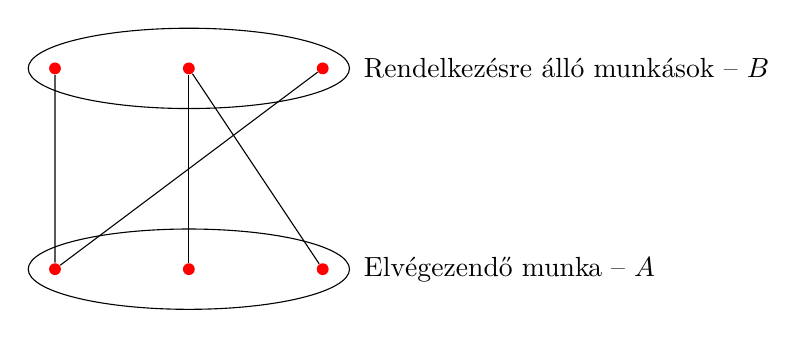
\begin{tikzpicture}[scale=1.7]
  \tikzset{ p/.style={circle,yellow,fill=red,inner sep=0pt,minimum size=0.15cm},
  }
 % the two sets
  \draw (0,0) ellipse (1.2cm and 0.3cm) node [right=2.1cm] {Elvégezendő munka -- $A$};
  \draw (0,1.5) ellipse (1.2cm and 0.3cm) node [right=2.1cm] {Rendelkezésre álló munkások --
  $B$};
  % the dots
  \node[p] (lB) at (-1, 0) {};
  \node[p] (lT) at (+1, 0) {}; 
  \node[p] (lC) at ( 0  , 0) {};
  
  \node[p] (rB) at (-1, 1.5) {}; 
  \node[p] (rT) at (+1, 1.5) {}; 
  \node[p] (rC) at ( 0, 1.5) {};
  
  % the connection between the dots
  \draw[-] (lT) -- (rC); 
  \draw[-] (lC) -- (rC); 
  \draw[-] (lB) -- (rB);
  \draw[-] (lB) -- (rT);
\end{tikzpicture} 
\end{figure}

Vékony Balázs

Gráf alakban megfogalmazva, adott $G=(V, E)$ gráf, ahol $V=(A, B)$ és $E=(x,y)$,
ahol $x \in A$ és $ y \in B$. Megkülönböztetünk $3$ fajta helyzetet:
\begin{description}
  \item[Maximális párosítás problémája] Ekkor azt szeretnénk, hogy a párosítások
  száma minél nagyobb legyen.
  \item[Maximális súlyú párosítás problémája] Itt létezik minden párosításnak
  egy jósági tényezője, egy súlya: $w:E\rightarrow\mathbb{R}$; egy adott $M$
  párosítás esetén $(M\subset E)$ keressük azt, amely maximális összeget ad:
  $\mbox{max}\left\{\sum_{e\in M}{w(e)}\right\}$.
  \item[Maximális teljes párosítás problémája] Most olyan párosítás halmazt
  keressünk, amely a lehető legtöbb párosítást létrehoz, a lehető legnagyobb
  összeggel. A teljes párositáshoz szükséges, hogy a vizsgált ponthalmaz páros
  legyen. Azt, hogy ez nem ekvivalens a korábbi feladattal
  \aref{fig:OptMaxNemEkv} ábra szemlélteti. Ekkor a maximális súlyú párosítást
  az $a_2-b_1$ adja, míg a maximális teljes párosítás problémájára a helyes
  válasz az $a_1-b_1$ és $a_2-b_2$ él párok.
\end{description}

\begin{figure}[htb]
\caption{Maximális súlyú és teljes párosítás probléma}
\label{fig:OptMaxNemEkv}
\centering
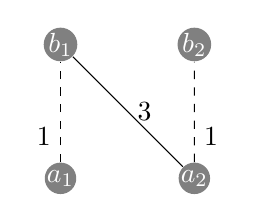
\begin{tikzpicture}[scale=1.7]
  \tikzset{
  p/.style={circle,white,fill=gray,inner sep=0pt,minimum size=0.15cm},
  }
  % the dots
  \node[p] (a1) at (0, 0) {$a_1$};
  \node[p] (a2) at (1,  0) {$a_2$};
    
  \node[p] (b1) at (0, 1) {$b_1$};
  \node[p] (b2) at (1,  1) {$b_2$};
    
  % the connection between the dots
  \draw[-] (a2) -- (b1) node [midway, right] {$3$};
  \draw[-,style=dashed] (a1) -- (b1) node [near start, left] {$1$};
  \draw[-,style=dashed] (a2) -- (b2) node [near start, right] {$1$};
\end{tikzpicture} 
\end{figure}

A maximális súlyú párosítás problémája \emph{visszavezethető} a maximális tejles
súlyú párosítás problémájára. A transzformációhoz a kevesebb csúcsú halmazt ($A$
és $B$ közül) egészítsük ki, hogy a két halmaz számossága megegyezen. Majd a
hiányzó és negatív súlyú éleken (a két halmazt közt) legyen $w=0$. 

\subsection{Magyar módszer}

Megoldás ad a maximális párosítás problémára polinomiális időben. Induljunk ki
bármilyen meglévő párositásból, egy ilyent \aref{fig:MagyModHelyeseg} ábra mutat
be.

\colorlet{ColorPink}{red!20}
\colorlet{ColorBlue}{blue!20}

\begin{figure}[htbp]
\caption{Magyar módszer helyessége}
\label{fig:MagyModHelyeseg}
\centering
\begin{tikzpicture}[font=\small,scale=1.7]
  \tikzset{
  p/.style={circle,white,fill=gray,inner sep=0pt,minimum size=0.15cm},
  }
  % the dots
  \draw[fill,ColorPink] (0.5,0) ellipse (0.7cm and 0.2cm) node [above=10pt,black] {$B_3$};
  \node[p] (B31) at (0,  0) {};
  \node[p] (B32) at (1,  0) {};
  
  \draw[fill,ColorBlue] (4,0) ellipse (1.5cm and 0.2cm) node [above=10pt,black] {$B_2$};
  \node[p] (B21) at (3,  0) {};
  \node[p] (B22) at (4,  0) {};
  \node[p] (B23) at (5,  0) {};
  
  \draw[fill,ColorPink] (7,0) ellipse (0.35cm and 0.2cm) node [above=10pt,black] {$B_1$};
  \node[p] (B11) at (7,  0) {};
  
  \node[p] (A31) at (0,  -1) {};
  \node[p] (A32) at (1,  -1) {};
  \draw (0.5,-1) ellipse (0.7cm and 0.2cm) node [below=10pt] {$A_3$};
  
  \draw[fill,lightgray] (4,-1) ellipse (1.5cm and 0.2cm) node [below=10pt,black] {$A_2$};
  \node[p] (A21) at (3,  -1) {};
  \node[p] (A22) at (4,  -1) {};
  \node[p] (A23) at (5,  -1) {};
  
  \draw[fill,lightgray] (7.5,-1) ellipse (0.7cm and 0.2cm) node [below=10pt,black] {$A_1$};
  \node[p] (A11) at (7,  -1) {};
  \node[p] (A12) at (8,  -1) {};
    
  \draw[-, color=blue, style=dashed] (A32) -- (B11);
  \draw[-, color=black, thick] (A31) -- (B31);
  \draw[-, color=black, thick] (A32) -- (B32);
  
  \draw[-, color=black, thick] (A21) -- (B21);
  \draw[-, color=black, thick] (A22) -- (B22);
  \draw[-, color=black, thick] (A23) -- (B23);
  
  \draw[-, color=green, thick] (A31) -- (B21);
  \draw[-, color=green, thick] (A32) -- (B31);
  \draw[-, color=green, thick] (A22) -- (B21);
  \draw[-, color=green, thick] (A22) -- (B23);
  
  \draw[-, color=green, thick] (B22) -- (A11);
  \draw[-, color=green, thick] (B23) -- (A12);
  
\end{tikzpicture} 
\end{figure} 

Egy ilyen gráfon végezzük el a következő definiciókat: 

\begin{description}
  \item[Alternáló út] olyan él sorozat (séta) amely $A$-ból indul és minden második 
  él párosításbeli.
  \item[Javító út] olyan alternáló út amely $B$-ben végződik.  
\end{description}

Ekkor a magyar módszer algoritmus lépései:

\begin{enumerate}
  \item Keresünk egy javító utat.
  \item Cseréljük meg az út menetén a szerepeket:
  	\begin{itemize}
  	\item párosításbeli élek kivétele,
  	\item nem párosításbeli élek betétele. 
	\end{itemize}
  \item Lépjünk, vissza az első lépéshez ameddig létezik javító út.
\end{enumerate}

Az algoritmus helyességének belátásához térjünk vissza \aref{fig:MagyModHelyeseg} ábrához,
amely egy köztes állapotot szemléltet. Legyen:
\begin{description}
  \item[$(A_1)$] -- azon csúcsok halmaza, amelyet az $M$ párosítás le nem fedett $A$--ban.
  \item[$(B_2)$] -- $A_1$--ből alternáló úton elérhető csúcsok halmaza,
  \item[$(A_2)$] -- $B_2$--hőz tartozó párosítás, 
\end{description}

Amennyiben az algoritmus leállt $B_2$ halmaz csúcsainak végpontja $A_2$ és $A_1$
halmazból induló élek, azaz $B_2$ lefogó pontja~\footnote{A lefogó ponthalmaz egy
adott G (rész)gráf minden élének legalább egyik végpontját tartalmazza.} az $A_1
\cup A_2$ halmaznak. Azaz elmondható, hogy $A_3$ és $B_2$ lefogó pontja a
gráfnak, ugyanakkor $A_3$ és $B_2$ elem--száma megegyezik a párosítás számával.
A \emph{König tétel}~\footnote{ A tétel Kőnig Dénestől származik. Legyen egy $G$
páros gráf, ekkor $\nu(G)=\tau(G)$ (azaz a legnagyobb független él halmaznak
ugyanannyi eleme van, mint a legkisebb lefogó pont halmaznak) és ha $G$--ben
nincs izolált pont akkor $\rho(G)=\alpha(G)$ (azaz a legkisebb lefogó él halmaz
azonos méretű a legnagyobb független pont halmazzal).} értelmében ezért a
párosítás maximális ($ |M|=|A_3 \cup B_2| \Rightarrow \nu(G) = \tau(G)$
-- |max független élhalmaz| = |min lefogó ponthalmaz|).

\subsection{Egerváry algoritmusa}

Az Egerváry~\footnote{Egerváry Jenő} algoritmus súlyozott páros gráfokra megadja
a maximális összsúlyú teljes párosítást. Ehhez az algoritmus először definiálja
a címkézés műveletet: minden csúcshoz rendel egy valós értéket ($c:V \rightarrow
\mathbb{R}$) úgy, hogy minden él pár esetén ($\forall \left\{x,y\right\} \in E |
x \in A, y \in B$) igaz a következő kifejezés: $c(x)+c(y) \geq w(e)$. Amennyiben
$c(x)+c(y)=w(e)$ legyen az él ,,piros.'' E címkézés mellet: $\sum_Mw(e) \leq
\sum_Vc(v)$, azaz a maximális összsúlyú teljes párosítás összsúlya kisebb, mint
a címkézés ősszege.

Bizonyítás, adódik a definicióból:

\begin{displaymath}
\sum_M{w} \leq \sum_M{\left[c(x)+c(y)\right]} = \sum_V{c(v)}
\end{displaymath}

\emph{Lemma}: Ha $M$--ben $\forall$ él piros, a párosítás maximális.

\subsection{Az algoritmus}

Vegyük továbbra is \aref{fig:MagyModHelyeseg} ábrát és az ott megfogalmazott definiciókat:

\begin{enumerate}
  \setcounter{enumi}{-1}
  \item lépés (inicializálás):   \begin{displaymath}
  c(v)=\begin{cases}
  \mbox{max}(w) & v \in A, \\
  0             & v \in B.
  \end{cases} 
  \end{displaymath}
  \item lépés: keressük meg a maximális elem--számú párosítást a piros részgráfban
  javító utakkal.
  Legyen ez a párosítás $M'$. Ha ez maximális megállunk.
  \item lépesben legyen:
  \begin{displaymath}
  \begin{rcases}
  x \in A_1 \cup A_2, \\
  y \in B_1 \cup B_3\\
  \{x,y\} \in E
  \end{rcases}
  \Rightarrow \sigma= min\left\{c(x) + c(y) - w(\left\{x,y\right\}) \right\},
  \end{displaymath}
  Majd: \begin{displaymath}
  c'(v)=\begin{cases}
  c(v)-\sigma & v \in A_1 \cup A_2, \\
  c(v)+\sigma & v \in B_2, \\
  c(v) 		   &  \mbox{másképp.}
  \end{cases} 
  \end{displaymath}
  Végül legyen $M=M'$ és $c=c'$ és folytassuk az első lépéstől.
\end{enumerate} 

Az algoritmus helyességének alátámasztásához be kell látnunk, hogy:

\begin{enumerate}
  \item A nulladik lépés címkézés.
  \item Létezik $\left\{x,y\right\}$ a második lépésben. Ez igaz, mert ha nem
  lenne akkor $A_1 \cup A_2$ bármely szomszédja $B_2$--ben volna és a
  \emph{Hall--feltétel} \footnote{$ \forall~x_0 \subseteq A$--ra az $|N(x_0)|
  \geq |x_0|$ egyenlőtlenségnek teljesülnie kell, másképp nem létezik párosítás
  ($N~x_0$ szomszédinak halmazát fedi).} alapján nem létezne párosítás 
  (mivel $|B_2| \geq |A_1 \cup A_2|$ nem teljesülne).
  \item $c'$ címkézés e? Ehhez figyeljük meg, hogy $\sigma$ hogyan változhat:
  
  \begin{tabular}{ l |  c c }
                  & $A_1 \cup A_2$ & $A_3$ \\
                  \hline
  $B_2$           & $0$            & $+\sigma$ \\
  $B_1 \cup B_3$ & $-\sigma$      & $0$ \\
  \end{tabular}
  
  Ugyanakkor a $\sigma > 0 $, hiszen $A_1 \cup A_2$ és $B_1 \cup B_3$ között
  vezető élek között nem lehet piros él. Tehát a címkézés csak egy helyt csökken
  (ami elronthatná a címkézést), de itt csak a maximális csökkenthető értékkel
  csökken, tehát a címkézés tulajdonsága megmarad.
 
  \item Ahol $\sigma$ minimális ott egy piros él keletkezik, ezáltal a piros
  részgráf is megváltozik. Ha az $\in B_1$ nő a párosítás mérete, mivel ha a
  párja $A_1$--ben van akkor simán összeköthető, ha meg $A2$--ben akkor az
  $A_1-B_2-A_2-B_1$ utón elérhető és ez hosszab mint az eredeti. 
  
  Ellenben, ha a piros él $B_3$--beli akkor $A_3$ és $B_2$ között megszűnik egy
  piros él, de ez nem befolyásolja a párositást, hiszen az új piros és $B_3$
  --beli végpontja elérhető lesz alternáló úton, ezért átkerül az $B_2$--be.
  
  Tehát $B_3$ legfeljebb $n$ lépésből elfogy. A  következő lépésben $B_1$--belli
  a piros él, tehát nő a párosítás $\Rightarrow n^2$ iterációba legfeljebb
  megvagyunk. Egy iteráció időigénye $O(e)$ (a $\sigma$ kiszámolása és $A_1 \cup
  A_2$ előállitása), tehát az algoritmus komplexitása $O(n^2e)$.
  \end{enumerate}